\documentclass[a4paper, oneside]{scrartcl}

%\usepackage{longtable}
%\usepackage{booktabs}
%\usepackage{a4wide}
\usepackage{graphicx}
\usepackage{caption}
\usepackage{subfig}
\usepackage{wrapfig}
\usepackage{verbatimbox}
\usepackage[activate={true,nocompatibility},final,tracking=true,kerning=true,spacing=true,factor=1100,stretch=10,shrink=10]{microtype}
\microtypecontext{spacing=nonfrench}
% activate={true,nocompatibility} - activate protrusion and expansion
% final - enable microtype; use "draft" to disable
% tracking=true, kerning=true, spacing=true - activate these techniques
% factor=1100 - add 10% to the protrusion amount (default is 1000)
% stretch=10, shrink=10 - reduce stretchability/shrinkability (default is 20/20)
\parskip=7pt
\parindent=0pt
%\usepackage{apacite}
%\usepackage{minted}
%\usepackage{listings}
\usepackage[utf8]{inputenc}
\usepackage[T1]{fontenc}
\usepackage[english]{babel}
\usepackage[hyphens]{url}
\usepackage[colorlinks, linkcolor=black, urlcolor=black, citecolor=black, pdfpagemode=UseNone, pdfstartview=]{hyperref}

\captionsetup{format=plain}

% ProVerif model style options
\newcommand{\kwl}[1]{\mathbf{#1}}
\newcommand{\kwf}[1]{\mathsf{#1}}
\newcommand{\kwc}[1]{\mathsf{#1}}
\newcommand{\kwp}[1]{\mathsf{#1}}
\newcommand{\kwt}[1]{\mathsf{#1}}
\newcommand{\kwe}[1]{\mathsf{#1}}
\newcommand{\kwtable}[1]{\mathsf{#1}}
\newcommand{\var}[1]{\mathit{#1}}

\author{Geert Smelt\thanks{\href{mailto:gasmelt@student.ru.nl}{\nolinkurl{gasmelt@student.ru.nl}}}}
\title{Verified IRMA Assurer}
\subtitle{Securely storing identity document chip data onto IRMA cards}
\date{\today}
\dedication{Kerckhoffs Institute\\Supervisor: Bart Jacobs}

\begin{document}
\maketitle

\begin{abstract}
\noindent
IRMA Assurer is an ideal method for new adopters of IRMA technology to obtain an initial set of Attribute Based Credentials using one's identity document such as a passport. Due to the nature of IRMA such an initialization is required to adhere to strict cryptographic rules. In this paper we describe the theory behind IRMA and passport security. Furthermore we specify guidelines which such a protocol has to follow and we design the Assurer protocol. We prove the soundness and cryptographic security of our protocol by creating a model of it in the Pi Calculus and running the ProVerif cryptographic protocol verifier on it.
\end{abstract}

\section{Introduction}

\subsection{Terminology}
Tablets, from here on simply called clients.
Attribute data cryptographically signed by the server, from here on simply called attribute data (signing is implied).
IRMA card, simply called card.
Identity document with embedded chip like driver's license, ID card or passport. Denoted as passport for simplicity.
Authentication with respect to IRMA cards means the card is presented to a terminal (e.g. in a supermarket) which verifies the card user has the required attributes (e.g. age $\geq$ 18) for purchasing items (e.g. alcohol).
IRMA Assurer protocol, simply called Assurer.

\subsection{Motivation}

\chapter{Theory}
\label{sec:theory}
This chapter describes the theory behind the two main actors of the protocol that Assurer aims to connect. We start by providing insight into the IRMA ecosystem, followed by an overview of the electronic passport's security measures. Afterwards we sketch a typical run of the IRMA card application process.

\section{IRMA}
Here we explain the background of the IRMA proofs. IRMA stands for I Reveal My Attributes, which is a reference to attribute-based credentials (ABC) as described by~\cite{zeroknowledgeprotocols,abcfortrust,alpar2013credential}. ABCs (sometimes also referred to as anonymous credentials) are a way for people to share a part of their digital identity without disclosing any other information irrelevant to the goal of authentication. A digital identity is generally considered to be a set of characteristics describing particular properties about an individual. A distinction is made between identifying and non-identifying ABCs. Identifying ABCs are typically date of birth, name and social security number, whereas non-identifying ABCs may include hair color or a favorite dish. Furthermore the set of ABCs is context-dependent and dynamic~\cite{abcofabc}. For the IRMA protocol only the identifying ABCs are relevant and use of the term ABC in the remainder of this document will refer only to this type.

In addition to the property it describes, any ABC is required to contain two additional basic attributes. First, an expiry date has to be determined at issuance, and it is included as an attribute applying to the whole credential. When the credential is verified, the expiry date can be revealed to confirm validity. Second, each user has a master secret key, stored in the smart card's secure storage, which is also incorporated -- technically, like an attribute -- in all credentials~\cite{alpar2013credential}.

Before it is possible to make use of ABCs for identification these first have to be provided by a third party, called an issuer. These issuers are parties who are allowed to give out ABCs. Any issuer cannot simply give out any ABC however. For example a bank may issue an ABC called `customer ID' for people who are customers with that particular bank, but may not issue credentials such as `date of birth' for the same people, or any other people for that matter. There are certain roles that issuers may assume and those they may not. Issuers determine the particular attributes they give out, but are verified by a scheme manager. Such a scheme manager effectively facilitates purpose limitation and data minimization.

To summarize, the ecosystem distinguishes four roles:
\begin{enumerate}
  \item \textbf{Users} are people who own a smart card that holds valid ABCs; validity means that the ABCs on the card are valid for the card holder (and are not expired).
  \item \textbf{Issuers} are the authorities that sign credentials with attributes and provide them to users. For  instance, citizen registration authorities are the obvious issuers of `over 18' ABCs (and of many other ABCs as well) and banks are authoritative issuers of bank account number ABCs.
  \item \textbf{Verifiers} (also called \textbf{relying parties}) are the parties that verify a subset of the available ABCs on a card in order to authorize a transaction. An example verifier is a website that wants to verify the ABC `over 18' before it allows viewing of a certain video online.
  \item The \textbf{scheme manager} is an independent, non-profit organization that sets the rules for the different parties (users, issuers and verifiers) and is responsible for the software and smart card management.
\end{enumerate}

Effectively an ABC can be seen as a secure container in which a characteristic from one's digital identity is stored. The attribute values are verified by issuer to ensure they match the individual's characteristics. Once a characteristic is verified the issuer will cryptographically sign the corresponding attribute and store it in the container. A municipality may for instance issue ABCs that state your place of birth and date of birth, which can then be checked by relying parties that require access to this information.

The benefit of using ABCs in favor of regular identification via say passports is the fact that it allows for selective disclosure of characteristics. This enhances the privacy of your (digital) identity by not revealing anything that is not strictly necessary. Consider the following example. You wish to rent a movie that contains violence. These movies typically require a minimum age. In the Netherlands such movies require you to be at least 18 years of age. When you wish to rent such a movie, the cashier asks you to prove you are at least 18 years old. ABCs allow you to digitally tell the cashier that you are `at least 18 years old' and are allowed to rent the movie. Note that the cashier never learns your actual age.

As stated above the IRMA project makes use of these ABCs, but mainly focuses on efficiency and practical issues when employing them~\cite{abcofabc}. All applicants receive a smart card that only features a photo of the card holder on the front. No further personally identifiable information is visible on the card.

An IRMA (smart) card is the physical container of attribute-based credentials. As you can see below, the card shows only a picture of its holder but no other personal data. This is important for privacy and security reasons.

\begin{figure}[!ht]
  \centering
  \subfloat[Front\label{subfig:irma-front}]{%
    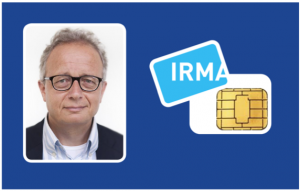
\includegraphics[width=0.45\textwidth]{images/IRMA_card_front.png}
  }
  \subfloat[Back\label{subfig:irma-back}]{%
    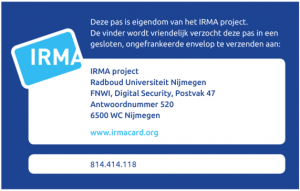
\includegraphics[width=0.45\textwidth]{images/IRMA_card_back.png}}
  \caption{IRMA card}
  \label{fig:dummy}
\end{figure}

\begin{enumerate}
	\item Your photo enables others to verify that the card belongs to you.
  \item In many situations it is not necessary to reveal your name or date of birth. That’s why they are not printed on the card. However, the card may contain these values digitally, stored as ABCs.
  \item On the back of the card there is a card number. This number is only used for card administration. For instance, when a new card is handed over to a user, it is easy to find it based on this number.
  \item The card number is not visible, but stored digitally inside the card.
\end{enumerate}

\section{Passport}
\label{subsec:passports}
\setlength{\columnsep}{16pt}
\begin{wrapfigure}{R}{0.3\textwidth}
  \centering
	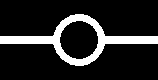
\includegraphics[width=0.2\textwidth]{images/biometrics_logo.pdf}
	\caption{Symbol to indicate a biometric passport}
	\label{fig:biometricslogo}
\end{wrapfigure}
The passport is a travel document issued by a country's government that certifies the identity and nationality of its holder for the purpose of international travel~\cite{passportdefinition}. A biometric passport is an upgraded version that contains biometric information that can be used to authenticate the identity of travelers. This information is stored on an embedded chip that can be read using contactless smart card technology. Passports that feature such a chip generally feature the symbol shown in figure~\ref{fig:biometricslogo} on the cover. The data stored on the passport chip needs to be protected from modification, cloning, eavesdropping, etc. For this purpose several protection mechanisms have been implemented. Each of these mechanisms exists alongside each other and protects against different types of attacks. This section provides a brief overview of the various security protocols supported by passports, i.e. PA, BAC, PACE, SM and AA as specified by ICAO as well as EAC as specified in by BSI~\cite{icao,bsi}. 

\subsection{Passive Authentication}
\setlength{\columnsep}{10pt}
\label{subsubsec:pa}
Passive Authentication (PA) is not actually a protocol. It simply indicates that the chip makes use of digital signatures of its data. PA involves the terminal reading the data and verifying both its hash and signature. PA is the only `protocol' that is ICAO mandatory; all other protocols are optional~\cite{mostowski2010electronic}.

\subsection{Basic Access Control}
Consider the case where a passport does not feature an RF chip. In this scenario privacy of the passport data is achieved by being able to keep the passport closed so nobody can read its data. With the addition of the RF chip this would no longer hold. Anyone with an RF reader (often called a terminal) is able to read the data on the chip if it is in close proximity. The solution to this problem is to protect the data with a key that the reader needs to know before being allowed to read the data. This is how the Basic Access Control (BAC) protocol works. BAC is essentially not required to be used by ePassports, but is strongly recommended. In the European Union however the use of BAC is mandatory~\cite{icao}. The key used for BAC is derived from three properties of the passport.
\begin{enumerate}
	\item The document number (usually 9 digits)
  \item The date of birth (formatted YYMMDD in Dutch passports)
  \item The document expiry date (formatted YYMMDD in Dutch passports)
\end{enumerate}
These three properties are part of the Machine Readable Zone (MRZ) that is printed in monospace at the bottom of the passport (see figure~\ref{fig:dutchpassport}). Also part of the MRZ is the Burger Service Nummer (BSN), which is equivalent to the social security number and uniquely identifies a Dutch citizen, but this number is not used for the key derivation for BAC. Combining the aforementioned properties eventually results in the key with which the reader may access the chip's data. Keep in mind the MRZ is not visible while the passport is closed and cannot be obtained without opening the passport~\cite{baceacpassports}. Strictly speaking the MRZ could be obtained from the citizen database, but additional security checks are in place before it can be accessed. The only method of transferring the MRZ to the reader is for the reader to either utilize optical character recognition (OCR) software or for the passport holder to manually enter the information into the reader. In either case the MRZ is transmitted via an out of band channel. After the key is used for authenticating the reader to the passport, all further communication is performed via an encrypted channel using a session key~\cite{icao}.

In some countries, e.g. the US, the chip is shielded by a very thin metal mesh that is integrated into the cover of the passport~\cite{encuspassports}. This prevents readers from accessing the chip without having the passport holder open his or her passport first.

\subsection{Supplemental Access Control}
Supplemental Access Control (SAC) was introduced by ICAO in 2009 for addressing BAC weaknesses. It was introduced as a supplement to BAC (for keeping compatibility), but will replace it in the future. In principle it is a set of security features, which specifies the Password Authenticated Connection Establishment (PACE) protocol~\cite{icao}. PACE is preferred over BAC if it is implemented by a passport. It also derives the session key from the MRZ, but also allows key derivation from the Card Access Number (CAN) that is also present on the front of passports. The protocol uses a weak password (possibly of low entropy), verifies the password, and generates cryptographically strong session keys. It is mandatory from December 2014 onwards~\cite{gemalto}.

The PACE protocol comprises four steps:
\begin{enumerate}
	\item The chip randomly chooses a random number, encrypts it with a key derived from the password and sends the encrypted random number to the terminal, where it is recovered.
  \item Both the chip and the terminal use a mapping function to map the random number to parameters for asymmetric cryptography. 
  \item The chip and the terminal perform a Diffie-Hellman protocol based on the parameters generated during step 2. 
  \item The chip and terminal derive session keys, which are confirmed by exchanging and checking the authentication tokens.
\end{enumerate}

\begin{figure}[htb]
	\centering
		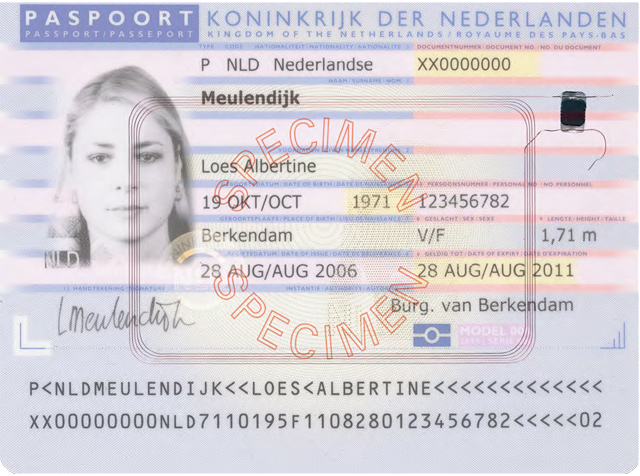
\includegraphics[width=0.50\textwidth]{images/dutchpassport.png}
	\caption{Dutch passport with a Machine Readable Zone}
	\label{fig:dutchpassport}
\end{figure}

\subsection{Secure Messaging}
The Secure Messaging (SM) protocol is used to protect the integrity and confidentiality of the communication between terminal and chip. Essentially the protocol sets up a secure channel, the key for which is agreed upon during the BAC or PACE protocol. When also performing EAC, the CA part will refresh the key (see below).

\subsection{Extended Access Control}
Starting in 2006 many countries added their citizens' finger prints and iris scans to the chip, by definition turning it into a biometric passport. In the Netherlands finger prints used to be stored for identity cards as well, but this decision was reverted and now only the passport holds the finger prints of Dutch citizens~\cite{idkaart}. The biometric data is a lot more sensitive than the data protected by BAC, meaning it needs to be protected by stronger cryptography. For this the Extended Access Control (EAC) protocol was developed and added to the second generation of ePassports in 2009~\cite{gemalto}. Any reader that has successfully performed BAC may subsequently perform EAC in order to obtain access to the finger print and iris of the passport holder. EAC is implemented in all new generation EU passports, but nowhere else.

EAC consists of two protocols, Chip Authentication (CA) and Terminal Authentication (TA), both relying on a public key infrastructure in which certificates are issued to the passport as well as other governments for verification purposes. The CA protocol is used for the terminal to authenticate the chip. It is based on a secret key agreement and a successful run of the protocol provides both parties with a new key for SM. The TA protocol is used for authenticating the terminal to the chip and possibly increase access rights. It actively verifies certificates. After both protocols have finished, mutual authentication is achieved and a new secure channel is created.

\subsection{Active Authentication}
Active Authentication (AA) is a challenge-response protocol that proves the authenticity of the chip, verifying the chip has not been cloned. The chip contains a private key, of which the chip proves knowledge during AA, and a certificate for this key as signed by the passport issuing country. This protocol is redundant when the passport also supports EAC, since the CA protocol also (implicitly) proves knowledge of this private key~\cite{secprivepassport}. This means that AA is only useful in cases where passports do not support EAC, but still wish to verify knowledge of the private key.

An example scenario of AA would be a passport that has a private key securely embedded in its chip. The public counterpart of this key is then signed by the passport's producer, Morpho\footnote{\url{http://www.morpho.com/}} in the Netherlands. Morpho's public key is subsequently signed by the Dutch government, creating a certificate chain. Sending a challenge to the chip, encrypted with its public key would allow the chip to solve the challenge by decrypting it using its private key and thus proving its identity to the terminal.

\section{Usage scenario}
\label{subsec:bcoe}
This section describes the basic course of events when a citizen requests a personal IRMA card and would like it to be initialized with his or her passport information. Here we only mention assumptions of operational nature. Goals and assumptions of cryptographic nature are discussed in chapter~\ref{sec:assumptions}. 

First of all we assume the citizen in question is an inhabitant of the Netherlands and is in possession of an electronic passport. The citizen will fill out an online application form and enclose a photo in order to request a new IRMA card. Once the application is received by the IRMA card manufacturer a new IRMA card will be created. This card is blank, i.e. there are no ABCs on the card. The application for this card, as well as the blank card itself, will subsequently be forwarded to one of several dozens of assurers. 

These assurers may be situated in a government building, for example in a town hall, or they could be notaries, they might be something else entirely as long as they are public figures who either directly or indirectly work for the government. Assurers are in possession of a tablet device that contains a Near-Field Communication (NFC) chip that allows for contactless communication with the IRMA card. This tablet will be kept under lock and key in a safe and is protected with a PIN in order to prevent unauthorized use. At each location only one person (a few at most) will be in posession of this key and PIN. The citizen will go to one of these assurers and present his or her passport to the tablet if the assurer confirms that the uploaded photo, which is printed on the front of the IRMA card, matches the citizen. 

The data on the passport is verified by the tablet and if confirmed to be valid will be sent to a (the only) central server. The server repeats these checks and also performs several additional checks to definitively verify the passport. Such additional checks may include absence of this particular passport in the database of stolen and lost passports. The server will then proceed to convert the passport's data into ABCs. These ABCs are cryptographically signed by the server, who is the only party in posession of the private part of the only attribute signing key pair, i.e. the issuer key pair. Once the passport data is converted into ABCs the server sends them back to the assurer's tablet. The server keeps a log of the passport number plus the time of the request, but deletes all other traces of the data (both passport and attribute) once it has been received by the assurer's tablet. 

The ABCs are received by the tablet and the assurer asks the citizen to present his or her IRMA card. The ABCs are subsequently written to the IRMA card by the tablet. Upon successful transfer of the ABCs, all traces of the entire transaction are deleted from the tablet. The citizen has now successfully added the data from his or her passport to the newly created IRMA card.

\chapter{Goals}
\label{sec:goals}
This chapter focuses on the goals of Assurer. We will describe the goals that should be met by the protocol and are going to be verified by means of a protocol prover. First and foremost, the protocol should ensure the clients will be authenticated to the server and vice versa. These properties should prevent susceptibility to man-in-the-middle attacks. Furthermore, both the all application data sent between client and server should be secret and trustworthy. Moreover, the protocol should be resistant against replay attacks targeting ABCs. Finally the protocol should be designed in such a way that the connection to the server will not cause a denial of service.

To summarize the protocol should offer:
\begin{itemize}
  \item authentication of client to server;
  \item authentication of server to client;
  \item integrity of passport data sent between server and client;
  \item confidentiality of passport data sent between server and client;
  \item integrity of ABCs sent between server, client and card;
  \item confidentiality of ABCs sent between server, client and card;
  \item resistance against replay attacks.
\end{itemize}

In addition, we wish to achieve perfect forward secrecy, meaning an attacker cannot derive previous session keys even if private keys are obtained (see chapter~\ref{subsubsec:pfs}). This means we have to use cryptographically strong keys, which also should be ephemeral.

Note that replay attacks are partly mitigated by policies surrounding the system. For example, replaying of ABCs is only possible should an attacker have access to the assurer's tablet, which is kept in a safe and is inaccessible. To improve upon this, implementations of the protocol should ensure it does not allow or facilitate storing ABCs internally for repeated use. All ABCs should be stored on the corresponding IRMA card and securely deleted immediately after.

\section{Attack scenarios}
This section describes possible attack scenarios with respect to the goals described above. These are attacks the protocol should be resistant against. The possible impact of such an attack is described directly after the attack itself, along with the likelihood of such an attack occurring.

\begin{itemize}
	\item An attacker reads the passport data sent between client and server. This attack causes personally identifiable information to be learned, leading to a breach in confidentiality. This may be likely in the event weak cryptography is used or if either party loses its key. However, because of the requirement of perfect forward secrecy this issue is partly mitigated (see section~\ref{subsubsec:pfs}).
  \item An attacker modifies the passport data sent between client and server. This attack causes the server to receive data inconsistent with the passport data sent by the client, at worst leading to the issuance of ABCs not corresponding to the passport. This can be mitigated, like the previous scenario, with the use of sufficiently strong cryptography, but is still somewhat likely to occur with a powerful adversary.
  \item An attacker modifies signed ABCs. This attack causes the client to receive incorrect ABCs, at worst leading to the issuance of ABCs not corresponding to the passport. This is highly unlikely as it would require the attacker to be able to sign the ABCs using the issuer's private key to keep relying parties from detecting the fraud.
  \item An attacker intercepts ABCs and stores it onto his own card. This attack causes false issuance of ABCs, in turn leading to possible fraud. This may be a likely scenario if the attacker controls the network and is actively attacking the protocol. A mitigating factor is the fact the attacker must first obtain access to the tablet, which as described is kept under lock and key.
  \item An attacker submits forged passport data to the server. This attack causes the server to possibly provide ABCs for fictitous people, in turn leading to possible fraud. Because the server verifies all passport data before providing ABCs, it may also be possible to query the server, guessing correct personally identifiable information.
  \item An attacker intercepts and later reuses ABCs already stored onto a card for storing on another card. This attack causes the attacker to be able to commit fraud. This is likely in the case where ABCs are not protected against replay attacks. In Assurer we make use of nonces to ensure timeliness, which should mitigate this issue.
  \item An attacker replays the sending of passport data to obtain another identical set of ABCs. This attack effectively facilitates the cloning of cards. Since the server is keeping a log of all of the ABCs that are given out a simple lookup would reveal the replay attack, making this an unlikely scenario.
  \item An attacker uses different ABCs from different people to authenticate. This attack allows combining ABCs to achieve the required combination for authentication. This is hardly an issue, due to the fact the IRMA card features a photo that should resemble the authenticating person. Adding to that the fact that switching cards midway would raise eyebrows leads us to think this attack is unlikely to occur.
  \item An attacker causes a denial of service on the client. This may cause clients to not receive the requested ABCs, causing them to restart the process. This does not lead to a security risk.
  \item An attacker causes a denial of service on the server. This halts all activity surrounding the issuance of ABCs, but does not lead to a security risk.
  \item An attacker shows up with someone else's passport. At worst this could cause incorrect ABCs to be placed onto an IRMA card, however this is mitigated by verifying the photograph printed on the passport. In order to pass this test the attacker has to forge the passport, which is detected upon verification by either the client or the server. This scenario is therefore unlikely.
  \item An attacker switches out the non-initialized IRMA cards before they reach the assurer's office. This also is a non-issue, because these cards only contain a unique ID at this point in the process. This ID is not used by the relying parties for verification of ABCs and therefore has no impact on the security and privacy of the system.
\end{itemize}

\subsection{Perfect Forward Secrecy}
\label{subsubsec:pfs}
In key exchange protocols there is a property called Perfect Forward Secrecy (PFS) that provides a more secure way of encryption with respect to everyday session encryption, because the key is deleted immediately after use and therefore cannot be stolen by an attacker or forced to be handed over by the government in an attempt to decrypt intercepted traffic~\cite{lecture2}. More specifically, the exposure of long-term keying material, used in the protocol to negotiate session keys, does not compromise the secrecy of session keys established before the exposure. This property is especially relevant to scenarios in which exchanged session keys require secrecy protection beyond their lifetime, such as in the case of session keys used for data encryption. This means it is relevant in Assurer, since a lot of sensitive information is being transfered and therefore needs to be kept secret.

The most common way to achieve PFS in a key-exchange protocol is by using the Diffie-Hellman key agreement with ephemeral exponents to establish the value of a session key, while confining the use of the longterm keys (such as private signature keys) to the purpose of authenticating the exchange (see authentication). One essential element for achieving PFS with the Diffie-Hellman exchange is the use of ephemeral exponents which are erased from memory as soon as the exchange is complete. This should include the erasure of any other information from which the value of these exponents can be derived such as the state of a pseudo-random generator used to compute these exponents~\cite{PFS}.

\section{Cryptographic properties}
To summarize the previous sections, the protocol should satisfy the following cryptographic properties.
\begin{itemize}
  \item Authenticity
  \item Accountability
  \item Confidentiality
  \item Integrity
  \item \scriptsize Availability
\end{itemize}


\chapter{Protocols}
\label{sec:protocols}
The IRMA Assurer protocol is an application level protocol. It is designed to run on top of TLS 1.2. Only the latest version of the TLS standard is considered cryptographically secure and therefore is the only version IRMA Assurer supports. A second argument for the use of version 1.2 is the possibility to achieve Perfect Forward Secrecy (PFS), meaning that in case the long term key is ever compromised, then the session keys derived from it before compromise are still secure~\cite{PFS}. This chapter will first describe the TLS protocol, explaining the chosen parameters. The IRMA Assurer protocol follows directly after.

\section{Transport Layer Security}
\begin{wrapfigure}{R}{0.46\textwidth}
  \centering
	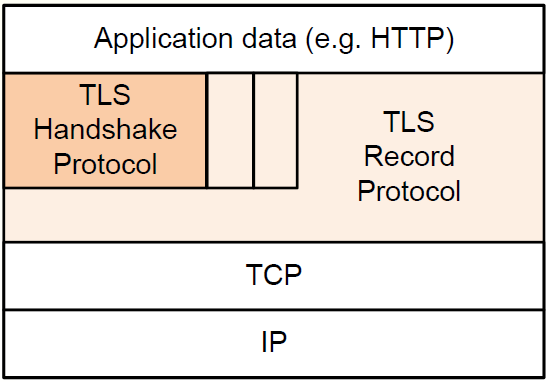
\includegraphics[width=0.4\textwidth]{images/tlsstack.png}
	\caption{TLS Protocol Hierarchy}
	\label{fig:tlsstack}
\end{wrapfigure}

The Transport Layer Security (TLS) protocol is a protocol operating on the presentation layer of the OSI Reference Model~\cite{osi}. It is a protocol that secures the connection between two parties across an insecure channel, ensuring secrecy~\cite{tls1.2}. It also has the possibility for authentication based on certificates. TLS is commonly used in web browsers to encrypt HTTP into HTTPS traffic, but it is capable of protecting any TCP connection~\cite{lecture}.

TLS 1.2 was defined in RFC 5246 in August 2008. It is based on the earlier TLS 1.1 specification. It was further refined in RFC 6176 in March 2011 removing their backward compatibility with SSL such that TLS sessions will never negotiate the use of Secure Sockets Layer (SSL) version 2.0.

The protocol consists of two major parts, TLS Handshake and TLS Record. Handshake is used for setting up connections between two parties, with optional authentication, while Record is used for ordering, encrypting and sending of the data. Handshake makes use of Record, so they work both alongside as well as on top of each other (see figure~\ref{fig:tlsstack}).



\subsection{TLS handshake}
Figure~\ref{fig:tlshandshake} shows a schematic overview of the TLS handshake, copied from RFC 5246~\cite{tls1.2}. An asterisk indicates a step necessary for client-to-server authentication. The handshake begins when a client connects to a TLS-enabled server requesting a secure connection and presents a list of supported cipher suites (ciphers and hash functions). From this list, the server picks a cipher and hash function that it also supports and notifies the client of the decision. The server usually then sends back its identification in the form of a digital certificate. The certificate usually contains the server name, the trusted certificate authority (CA) and the server's public encryption key. The client may contact the server that issued the certificate (the trusted CA) and confirm the validity of the certificate before proceeding. In order to generate the session keys used for the secure connection, the client encrypts a random number with the server's public key and sends the result to the server. Only the server should be able to decrypt it, with its private key. From the random number, both parties generate a 'master secret' and then negotiate a session key for encryption and decryption.

The details about the underlying cryptographic functions selected for the IRMA Assurer protocol, such as encryption and hashing functions will be discussed later in section~\ref{sec:assumptions}.

\begin{verbbox}
Client                                               Server
------                                              -------
ClientHello              -------->
                                                ServerHello
                                               Certificate*
                                         ServerKeyExchange*
                                        CertificateRequest*
                         <--------          ServerHelloDone
Certificate*
ClientKeyExchange
CertificateVerify*
[ChangeCipherSpec]
Finished                 -------->
                                         [ChangeCipherSpec]
                         <--------                 Finished
Application Data         <------->         Application Data
\end{verbbox}

\begin{figure}[htb]
\centering
\theverbbox
\caption{TLS Handshake}
\label{fig:tlshandshake}
\end{figure}

TLS also supports extensions. These are additional supported features, each with its own specification~\cite{tlsext}. These extensions can be used in either party's Hello message to indicate special wishes. This is useful to upgrade the TLS connection to a more secure version by increasing the minimum recommended cryptographic parameters. For example, TLS in its basic form is vulnerable to a handshake renegotiation attack~\cite{lecture}. In essence an attacker may send arbitrary data followed by a renegotiation intercepted from a regular client to trick a server into believing the arbitrary data was sent by this client instead. An extension has been developed to combat this, which is described in RFC 5746~\cite{tls_handshake_vuln}. We assume this extension to be used on every handshake performed during runs of Assurer and do not explicitly mention it in the following sections.

\subsection{TLS record}
The record protocol handles the sending and receiving of TLS related messages. It forms the basis of the TLS protocol. When sending, it will split the data in blocks, optionally compress it, apply a MAC, encrypt the data, add a fragment header and finally send the data over TCP port 443. When receiving, it will decrypt the data, verify the MAC, optionally decompress, defragment and finally deliver the data to the upper layer. Essentially this protocol forms the secure channel between client and server~\cite{tls1.2}.

\section{IRMA Assurer}
The IRMA Assurer protocol makes use of TLS 1.2 as described above. This means both the server and the tablets will verify each other's certificates and agree upon a session key. Once a secure channel has been successfully set up, we have achieved privacy and data integrity of all communication over this channel~\cite{tls1.2}.

After the secure channel is established the application data is transferred between client and server. This entails the sending of the passport data from the client to the server, followed by the sending of ABCs from the server to the client. Before passport data can be sent however, the client needs to read the chip that is present in the passport using special software and hardware. For the purpose of this protocol we assume the client has already performed this action and has knowledge of the passport data.

Shown in figure~\ref{fig:assurer} is the Assurer protocol using the informal Alice-Bob notation. Lines that are not numbered indicate an action outside of the scope of the protocol or an assumption that needs to hold before the next line can be executed. In this notation we denote the client by \texttt{A} and the server by \texttt{B}. Note that the Active Authentication steps do not involve the client as it only forwards communication to and from the passport, denoted by \texttt{P}. Furthermore, \texttt{skP} indicates the private key stored inside the passport and \texttt{kAB} is the key that is agreed upon during the handshake.

\begin{verbbox}
   [Citizen presents passport]
   [Client performs PA]
1. A --> B: ClientHello
2. B --> A: ServerHello, Certificate, ServerKeyExchange, 
            CertificateRequest, ServerHelloDone
3. A --> B: Certificate, ClientKeyExchange, CertificateVerify, 
            ChangeCipherSpec, {Finished}kAB
4. B --> A: ChangeCipherSpec, {Finished}kAB
5. A --> B: {{Passport, A, B, Na}kAB, #{Passport}kAB}kAB
   [Server performs PA]  
6. B --> A --> P: {Nb}kAB
7. P --> A --> B: {{Nb}skP}kAB
   [Server verifies response to AA challenge]  
8. B --> A: {{ABCs, A, B, Na}kAB, #{ABCs}kAB}kAB
   [Client stores ABCs on IRMA card]
\end{verbbox}

\begin{figure}[htb]
\centering
\theverbbox
\caption{IRMA Assurer including TLS handshake}
\label{fig:assurer}
\end{figure}

\subsection{Assumptions}
\label{sec:assumptions}
In this section we discuss the assumptions made with regard to Assurer. The section is divided into two parts. The first section discusses assumptions on the operational level and the second describes assumptions with respect to cryptography.

\subsubsection{Operational}
Operational assumptions mostly focus on procedures that have to be followed for the Assurer protocol to work. We reiterate some parts of the basic course of events described in section~\ref{subsec:bcoe} to make them explicit as assumptions. 

The entire ecosystem in which Assurer operates can be described as a star structure. At the center of the star will be the (only) server. The edges (points) of the star are formed by the clients. Clients do not communicate with each other, but only with the server. Each of these clients has their own NFC-enabled tablet, which is locked up in a safe and PIN code protected to prevent malicious use. By using an Android app installed on these tablets assurers may access data on passport chips and IRMA cards. Upon client initialization this app is installed on the tablet, as well as the fully qualified domain name (FQDN) of the server. By using the FQDN the server has the option to switch IP addresses without breaking the system. Also installed on the tablet are a client certificate (signed by the server) required for authentication and its corresponding private key. The server checks the certificate for validity and also checks if it has not been revoked by accessing Certificate Revocation Lists (CRL), which mitigates issues with stolen tablets or misuse. Finally the public key of the server is installed for easy access.

Although subject to change, at the time of writing the communication between IRMA card and terminal, i.e. tablet, is still being sent in the clear. Upon reading data from a passport chip the integrity is verified by the client by executing BAC and PA, and sent to the server for further analysis. The server performs the same checks, plus AA, and looks up the person corresponding to the data in a central database. If everything is proven to be valid the server will create digitally signed attribute-based credentials that correspond to the passport data. The server will then send these ABCs to the client, who will in turn install them on the person's IRMA card. Upon successful installation onto the IRMA card, the ABCs are securely deleted from both server and client. Furthermore, the passport data is securely deleted from the server and client. However the server does keep a log of the passport number that was part of the attribute signing request sent by the client, along with a timestamp. This facilitates traceability in case of anomalies. Finally, we do not support TLS session resuming. This property allows clients to send a stored session identifier to the server and then pick up where left off. Supporting this weakens the strength of the TLS connection, in particular the PFS property of TLS~\cite{tlssesres}. Since we wish to have PFS we do not allow session resuming.

\subsubsection{Cryptographic}
Before going into the cryptographic choices regarding Assurer it is important to take a quick look at the transport layer used below. There are two options, the User Datagram Protocol (UDP) and the Transport Control Protocol (TCP). We have chosen to make use of TCP for the transport layer protocol. The main reason for this is that we require the packets to be delivered without packet loss. In other words, we favor TCP over UDP for its high reliability~\cite{tcp}. Furthermore it is best compatible with the TLS protocol which we aim to use. Other arguments for choosing TCP include its data flow control and packet reordering capabilities.

In order to achieve the goals described in section~\ref{sec:goals} several choices have been made regarding the cryptography. What follows is an argumentation for the decisions made for Assurer. 

The guideline for choosing supported cipher suites is to offer perfect forward secrecy. Any cipher suites that offer PFS capabilities have been selected, while suites that do not are not selected. In principle, any public key encryption scheme can be used to build a key exchange with PFS by using the encryption scheme with ephemeral public and private keys~\cite{PFS}. This means we have the option to use any public key infrastructure as long as we throw away the keys when we're done using them. Furthermore we can either choose elliptic curve cryptography or conventional cryptography. Because we wish to achieve mutual authentication both parties need to exchange certificates. These certificates must be of type X.509v3 in accordance with the TLS specifications~\cite{tls1.2}. The type of cryptography used for these certificates may either be RSA or DSA. Generally, in terms of performance, neither is significantly better than the other, meaning we may support both. 

As explained above we have chosen TLS 1.2 as basis for Assurer for its resistance against publicly known feasible attacks, as well as for its Perfect Forward Secrecy capabilities. This requires that the key generation for the encryption scheme must be fast enough. For most applications this disqualifies, for example, the use of ephemeral RSA public key encryption for achieving PFS, since the latter requires the generation of two long prime numbers for each exchange, a relatively costly operation~\cite{PFS}. For this reason we have selected the Diffie-Hellman Key Exchange protocol. Furthermore because of the faster key generation, better performance and shorter key length while still achieving the same level of security we have chosen to use elliptic curves~\cite{nsaecc}.

Since Assurer is to be used only on newly developed hardware and software it is safe to use the newest cryptography; there should not be any compatibility issues. Mozilla lists the following as the best choice for modern clients in their documentation on server-side TLS~\cite{mozilla}. The list is ordered from most recommended to least recommended. An exclamation mark indicates a technique which is forbidden.
%\def\hyph{-\penalty0\hskip0pt\relax}
\begin{description}
	\item [Ciphersuite] ECDHE-RSA-AES128-GCM-SHA256, ECDHE-ECDSA-AES128-GCM-SHA256, ECDHE-RSA-AES256-GCM-SHA384, ECDHE-ECDSA-AES256-GCM-SHA384, DHE-RSA-AES128-GCM-SHA256, DHE-DSS-AES128-GCM-SHA256, kEDH+AESGCM, ECDHE-RSA-AES128-SHA256, ECDHE-ECDSA-AES128-SHA256, ECDHE-RSA-AES128-SHA, ECDHE-ECDSA-AES128-SHA, ECDHE-RSA-AES256-SHA384, ECDHE-ECDSA-AES256-SHA384, ECDHE-RSA-AES256-SHA, ECDHE-ECDSA-AES256-SHA, DHE-RSA-AES128-SHA256, DHE-RSA-AES128-SHA, DHE-DSS-AES128-SHA256,DHE-RSA-AES256-SHA256, DHE-DSS-AES256-SHA, DHE-RSA-AES256-SHA, !aNULL, !eNULL, !EXPORT, !DES, !RC4, !3DES, !MD5, !PSK
  \item [Versions] \texttt{TLSv1.1, TLSv1.2}
  \item [RSA key size] \texttt{2048}
  \item [DH Parameter size] \texttt{2048}
  \item [Elliptic curves] \texttt{secp256r1, secp384r1, secp521r1} (at a minimum)
  \item [Certificate signature] \texttt{SHA-256}
  \item [HSTS] \texttt{max-age=15724800}
\end{description}

Note that this is the optimal configuration for Mozilla's own servers providing HTTPS connections, which explains the mention of HSTS. For the Assurer protocol we are only interested in cipher suites supported in TLS 1.2, while making use of elliptic curves and Diffie-Hellman, meaning we can safely ignore anything that is unrelated. Cross-referencing this list of cipher suites with the list of elliptic curve and TLS 1.2 cipher suites described by the OpenSSL documentation yields the following list of cipher suites supported by the Assurer, in descending order of priority~\cite{openssl}. These are named following IANA guidelines, which differs from the naming convention used by Mozilla who use OpenSSL guidelines, but is in correspondence with the RFC documents on TLS~\cite{tlsparams}. The blank lines indicate Mozilla favors either one or more non-elliptic curves or TLS 1.2 incompatible cipher suites over the ones that follow. 

\begin{verbatim}
TLS_ECDHE_RSA_WITH_AES_128_GCM_SHA256
TLS_ECDHE_ECDSA_WITH_AES_128_GCM_SHA256
TLS_ECDHE_RSA_WITH_AES_256_GCM_SHA384
TLS_ECDHE_ECDSA_WITH_AES_256_GCM_SHA384

TLS_ECDHE_RSA_WITH_AES_128_CBC_SHA256
TLS_ECDHE_ECDSA_WITH_AES_128_CBC_SHA256

TLS_ECDHE_RSA_WITH_AES_256_CBC_SHA384
TLS_ECDHE_ECDSA_WITH_AES_256_CBC_SHA384
\end{verbatim}

There are many reasons for this particular ordering. We highlight the main reasons below. 

\begin{itemize}
  \item Ciphers making use of ECDHE featuring AES in Galois Counter Mode (GCM) are selected first. These are TLS 1.2 ciphers and not widely supported at the moment. No known attack currently targets these ciphers.
  \item PFS ciphersuites are preferred, with ECDHE first, then DHE.
	\item ECDHE provides faster handshakes than DHE~\cite{bernat2011ssl,pfsprice}.
  \item AES 128 is preferred to AES 256, because it provides good security, is really fast, and seems to be more resistant to timing attacks.
  \item SHA256 is favored over SHA384. This appears to be mainly for interoperability purposes.
\end{itemize}

Galois Counter Mode (GCM) is an Authenticated Encryption (AE) algorithm. AE algorithms are designed to provide both data authenticity (integrity) and confidentiality. Since both are goals of Assurer we favor GCM over CBC, but do not require it.

For more information about the reasons behind this ordering please see~\cite{mozilla}. In August 2015 the NSA has issued a new version of their Suite B Cryptography document, in which they withdraw P-256, SHA-256, and AES-128 in order to start the transition to quantum resistant algorithms~\cite{nsacrypto}. Mozilla however does not yet have an updated document.

\subsubsection{Diffie-Hellman parameters}
Unfortunately, some widely used clients lack support for ECDHE and must then rely on DHE to provide perfect forward secrecy. This is true for Android $< 3.0.0$, Java $< 7$ and OpenSSL $< 1.0.0$, among others. Nowadays many, if not all, devices run Android versions higher than 3.0.0, so we don't expect to see issues here. However the Java requirement could lead to issues when implementing Assurer as an Android app, mainly because of the many IRMA-related dependencies that such an app has to deal with. These dependencies may not support Java 7 or 8 yet. Adding to that, Java 6 and 7 do not support Diffie-Hellman parameters larger than 1024 bits. This has consequences for the PFS requirement of Assurer. The only way a secure connection can be achieved from a Java 6 client is to use DHE cipher suites and use 1024-bit groups.

Use of the most widely used 1024-bit pre-computed Oakley group 2, standardized in~\cite{ike}, is considered unsafe, mainly because it is very likely that a state-level adversary may have broken it. In any case it is recommended to generate a random DH group instead of using a standardized one when setting up a new server~\cite{logjam}.

CBC ciphers can be attacked with the Lucky Thirteen attack if the library is not written carefully to eliminate timing side channels. This attack requires multiple sessions and is possibly detectable due to the low volume of traffic in Assurer. The attack is mitigated by use of a reasonably up-to-date cryptographic library, i.e. a library released anytime after March 2013. Most of the industry's libraries have released patches throughout February 2013, which probably makes this a non-issue for Assurer~\cite{lucky13}.

\paragraph{Logjam}
When choosing this list of supported cipher suites we have chosen the ``modern'' preset described by Mozilla. This is especially important, because of the recently discovered Logjam attack on the Diffie-Hellman key agreement, in particular within TLS, SSH and VPN connections~\cite{logjam}. Essentially Logjam is a type of attack that allows an attacker to downgrade the security of the connection to DHE export cipher suites. It is also possible to attack weak ($\leq$ 1024-bit) Diffie-Hellman groups by precomputing the group and then using it for lookups. The short term solution for mitigating Logjam attacks is for servers to disable export ciphers and use freshly generated groups of 2048 bits or larger. Clients should no longer accept groups of sizes lower than 1024 bits. In the long term however it is preferable to switch to elliptic curve cryptography (ECC) and not allow any other cipher suites. This is because none of the attacks presented work against ECC. As described above the Assurer protocol only makes use of a subset of the ``modern'' preset, which in turn only makes use of ECC cipher suites, and therefore is not susceptible to the Logjam attack.

\paragraph{Elliptic curves}
NIST has defined 15 standard curves~\cite{dss}. However, in practice, many implementations only support two of them, P-256 and P-384, because that is what the NSA recommends. As seen above Mozilla recommends to use at the very least P-256, P-384 and P-521. For Assurer we will follow that recommendation.

\subsubsection{Certificates}
\begin{itemize}
	\item Each client posesses one certificate, signed by the server, with which it may authenticate to the server. This occurs during the run of the TLS handshake protocol.
  \item Each passport contains one certificate with which the authenticity may be verified (see section~\ref{subsec:passports}).
\end{itemize}

\subsubsection{Keys}
The server owns two keypairs. The first keypair is used for signing and verification of certificates while the second one is used for the issuing and verification of attribute based credentials. A client only owns one keypair, which is used for signing and verification of certificates. The server's public key used for signing and verification is pre-loaded onto the clients during initialization, while the clients' public keys are stored within the pre-loaded certificates.

The use of TLS 1.2 with the aforementioned cryptographic options for the handshake will result in a symmetric session key held by both parties. From this point onwards we therefore have a secure channel to use for application data transfer.

\subsection{Application data}
All application data is protected with the session key as generated by the TLS handshake protocol. This ensures the passport and attribute data are sent over a secure channel. Once this channel has been established the client sends the passport data, including both parties' name and a fresh nonce, encrypted with the session key. Note that this is the same session key negotiated by the TLS handshake, meaning the passport data is essentially encrypted twice. Passive Authentication is then performed by the server. This is a double-check and consequently serves as verification that the client is not malicious. As described in section~\ref{subsubsec:pa} PA is ICAO mandatory and involves verification of the hash stored in the SOD file to ensure data integrity. After the integrity of the passport is verified the server continues with Active Authentication. For this it sends a challenge to the passport via the client, which has to be solved by the passport. The passport proves knowledge of a private key by signing the AA challenge using this key, which can in turn be verified by the server using the public key that was included with the passport data sent to the server during PA.

After both PA and AA have been performed the server will proceed with generating attribute based credentials that resemble the passport data. These ABCs are signed using the issuer key and combined with the names and nonce received during PA. This data is then encrypted and an HMAC is computed, both once again using the same session key, following which the data is sent to the client. The client checks the HMAC and decrypts the data. If the nonce and both parties' name matches the client will store the ABCs on the IRMA card. If the nonce does not match this may indicate a replay attack. If either party's name is incorrect this may indicate a man-in-the-middle attack. In both cases no attributes will be stored on the IRMA card and the protocol will halt.

\section{Formalisation}
\label{sec:formalisation}
In this section we describe the formalisation of the assumptions and use cases into a model written in the Pi Calculus. This model can be proven to be cryptographically secure using ProVerif. The model is listed in appendix~\ref{app:model}. This model is based on the TLS handshake model by Tankink and Vullers~\cite{tankink2008verification}. Their model makes use of RSA for the key exchange, but our model uses Diffie-Hellman. Similarly to their model we make use of message tagging, as is generally considered good practice. Furthermore, ProVerif has trouble finding attacks on variables that are being computed instead of being declared. Tankink and Vullers solve this by creating a new flag variable and outputting this on the supposed-to-be secret. This way when an attacker is able to obtain the flag, then he must have knowledge of the secret and an attack trace can be found. Furthermore we have added dead code checks to the model. This helps determine if the model fails midway. Such a failure is indicated by the fact that no falsification is found by ProVerif. Finally ProVerif appears to have a set a limit on the amount of RAM that it may use. It will not use more than 2GB of RAM, even though plenty is still available, and will consequently report a fatal error. To work around this, we have chosen to split the model into two parts: the first part describes the TLS handshake, while the second part describes the application protocol.

The model consists of three distinct phases. During the first phase the TLS handshake protocol is executed. As explained before we make use of an ephemeral Diffie-Hellman key agreement. This means that in this protocol the only use for both parties' keypair is the signing and verification of messages sent during the key agreement. Because of the nature of Diffie-Hellman, i.e. the Discrete Logarith Problem (DLP), it is not required to encrypt the protocol parameters as they can be sent in the clear without risk of an eavesdropper learning the agreed upon key. For authentication purposes however, we do require these protocol parameters to be signed by the sending party. This allows the receiving party to verify the identity of the sender before starting an encrypted session.

The second phase starts the actual Assurer application protocol, which takes place over the encrypted channel for which the key was negotiated during the TLS handshake of phase one. During this phase the passport is verified on the client's side by using passive authentication. This is done by checking the hash stored in the Security Object file of all the data groups contained within the passport. Once the client is confident that the integrity of the passport holds it proceeds by sending the passport data, plus a fresh nonce, to the server via the encrypted channel. The server will then also perform passive authentication as a double-check. If the server agrees with the client on the integrity of the passport, active authentication is performed. To do this, it sends a challenge that the passport has to solve. The passport has to sign this challenge in order to prove it has knowledge of the embedded private key. During passive authentication the server has obtained the passport's public key, which is used to verify the response to the challenge.

The third and final phase of the protocol is where the issuing of the Attribute Based Credentials takes place. As mentioned before the server is the only party that posesses the issuer private key. Every verifier, i.e. a terminal, for example at a supermarket has knowledge of the issuer's public key and is therefore able to verify the signature placed on the ABCs. The issuer's public key is not used in this model, as attribute verification is not included in its scope. The server creates ABCs and encrypts these ABCs, along with the nonce sent by the client during phase two as well as both parties' names, using the session key and computes an HMAC over the result. The encrypted data and its HMAC are sent to the client, which in turn verifies the HMAC and decrypts the data. If the decrypted data is found to match the nonce and the names of both parties, the client accepts the ABCs and stores them onto the IRMA card and closes the session.


\subsection{Discussion}
\textsc{TODO: Explain line by line what the model does}

\textsc{TODO: Look back on the goals and explain if they are met}
\chapter{Conclusion}
\label{sec:conclusion}
We have developed Assurer, a protocol for migrating personally identifiable information from identity documents to attribute-based credentials on IRMA cards. For this we have set several cryptographic goals and made assumptions regarding the use of the protocol. The protocol should satisfy authenticity, accountability, confidentiality, integrity and availability.

We have set out to prove these goals hold under the assumptions made, a task for which it is required to create a model of our protocol in the Pi Calculus and subsequently verify it using the ProVerif cryptographic protocol verifier. The creation of such a model has proven to be an error-prone task, mainly due to the limited amount of available literature on the subject, but also due to memory limitations of the software used. Thankfully, with the help of Jerry den Hartog, assistant professor in the security group at Eindhoven University of Technology, as well as Bruno Blanchet, head of research at the INRIA research institution, it was possible to overcome these issues. 

Using ProVerif we have provided proof that all of our goals, save availability, are met by the protocol. Since availability in our case constitutes only of the rule that clients must not cause an amount of traffic sufficiently high as to cause a denial of service on the server side. Unlike the other goals this is not really a cryptographic requirement, but instead more of a usability requirement, meaning we cannot use ProVerif for proof that this goal is satisfied. 

\section{Future work}
\label{sec:futurework}
The client in this protocol performs the task of storing the ABCs received from the server on a citizen's IRMA card. While several checks are performed to ensure honesty of clients this may still be undesirable. One would probably wish for less possible interference with the ABC data. Future work on this protocol might focus on making the transaction process of ABCs more opaque to the client, who would then only serve as a non-transparent tunnel through which the data is flowing. This in turn would mean the IRMA logic has to be moved from the client to the server, undoubtedly presenting new challenges.

Furthermore, at the time of writing the communication between IRMA card and the terminal is still being sent in the clear, i.e. without any cryptography. A valueable addition obviously would be to improve upon this area by creating a secure channel, which in fact would be a requirement for making the transaction process opaque as described above.

Finally one might wish to use this protocol for a software implementation. Due to the nature of IRMA and its implementations it is advisable to use Java for this. I have developed a prototype implementation of the protocol in order to get a good feel for the issues at hand. This implementation however remains unfinished, because it is now partly obsolete with the availability of IRMA's self-enrollment option via smart phones.


\nocite{*}
\bibliographystyle{plain}
\bibliography{references}

\clearpage
\appendix
\chapter{Model}
\label{app:model}
%\setlength{\thickmuskip}{0mu}

\section{Definitions}
\begin{Verbatim}[commandchars=\\\{\}]
\kwcom{(* A public channel *)}
\kwl{free} \kwc{net}.

\kwcom{(* Message tags *)}
\kwl{free} \kwc{ClientHello}, \kwc{ClientCertificateRequest}, \kwc{ClientCertificate}, 
     \kwc{ClientKeyExchange}, \kwc{CertificateVerify}, \kwc{ClientChangeCipherSpec}, 
     \kwc{ClientFinished}.
\kwl{free} \kwc{ServerHello}, \kwc{ServerCertificate}, \kwc{ServerKeyExchange}, \kwc{ServerHelloDone}, 
     \kwc{ServerChangeCipherSpec}, \kwc{ServerFinished}.
\kwl{free} \kwc{ClientPassport}, \kwc{ActiveAuthenticationChallenge}, 
     \kwc{ActiveAuthenticationReponse}.

\kwcom{(* Agent initialization is done over a private channel *)}
\kwl{private} \kwl{free} \kwc{clientInit}, \kwc{serverInit}, \kwc{initChannel}.

\kwcom{(* Initialization functions *)}
\kwl{private} \kwl{fun} \kwf{cert}/2.     \kwcom{(* Generating certificates for agents *)}
\kwl{private} \kwl{fun} \kwf{keypair}/1.  \kwcom{(* Generating assymmetric keypairs for agents *)}

\kwt{(** The cryptographic constructors **)}
\kwl{fun} \kwf{hash}/1.             \kwcom{(* Hashing *)}
\kwl{fun} \kwf{hmac}/2.             \kwcom{(* Keyed-hash message authentication code *)}
\kwl{fun} \kwf{encrypt}/2.          \kwcom{(* Symmetric key encryption *)}
\kwl{fun} \kwf{sign}/2.             \kwcom{(* Public key signing *)}
\kwl{fun} \kwf{sk}/1.               \kwcom{(* Extracts secret key of a keypair *)}
\kwl{fun} \kwf{pk}/1.               \kwcom{(* Extracts public part of a keypair *)}

\kwcom{(* The cryptographic destructors *)}
\kwcom{(* symmetric key decryption *)}
\kwl{reduc} \kwf{decrypt}(\kwf{encrypt}(\var{x}, \var{y}), \var{y}) = \var{x}.
\kwcom{(* signature verification *)}
\kwl{reduc} \kwf{unsign}(\kwf{sign}(\var{x}, \kwf{sk}(\var{y})), \kwf{pk}(\var{y})) = \var{x}.
\kwcom{(* verification of the agent as owner of the}
   \kwcom{key and retrieving the key from the certificate *)}
\kwl{reduc} \kwf{verify}(\kwf{cert}(\var{x}, \var{y}), \var{x}) = \var{y}.

\kwcom{(* Pseudo-random-number function for generating TLS session key}
   \kwcom{randomness *)}
\kwl{fun} \kwf{PRF}/1.

\kwcom{(* Symmetric key construction *)}
\kwl{fun} \kwf{clientK}/3.
\kwl{fun} \kwf{serverK}/3.

\kwcom{(* Diffie-Hellman computations *)}
\kwl{fun} \kwf{G}/0.                \kwcom{(* Generator point of the group *)}
\kwl{fun} \kwf{sm}/2.               \kwcom{(* Scalar multiplication *)}
\kwcom{(* Equality property: x . yG = y . xG *)}
\kwl{equation} \kwf{sm}(\var{y}, \kwf{sm}(\var{x}, \kwf{G})) = \kwf{sm}(\var{x}, \kwf{sm}(\var{y}, \kwf{G})).
\end{Verbatim}

\section{Queries}
\begin{Verbatim}[commandchars=\\\{\},codes={\catcode`$=3}]
\kwcom{(* secrecy secure channel *)}
\kwl{private} \kwl{free} \kwc{Sa}.
\kwl{private} \kwl{free} \kwc{Sb}.
\kwl{query} \var{attacker}{:} \kwc{Sa}.
\kwl{query} \var{attacker}{:} \kwc{Sb}.

\kwcom{(* secrecy passport *)}
\kwl{private} \kwl{free} \kwc{passportFlag}.
\kwl{query} \var{attacker}{:} \kwc{passportFlag}.

\kwcom{(* secrecy ABCs *)}
\kwl{private} \kwl{free} \kwc{abcFlag}.
\kwl{query} \var{attacker}{:} \kwc{abcFlag}.

\kwcom{(* secrecy Pre Master secret *)}
\kwl{private} \kwl{free} \kwc{PMSa}.
\kwl{private} \kwl{free} \kwc{PMSb}.
\kwl{query} \var{attacker}{:} \kwc{PMSa}.
\kwl{query} \var{attacker}{:} \kwc{PMSb}.

\kwcom{(* secrecy Master secret *)}
\kwl{private} \kwl{free} \kwc{MSa}.
\kwl{private} \kwl{free} \kwc{MSb}.
\kwl{query} \var{attacker}{:} \kwc{MSa}.
\kwl{query} \var{attacker}{:} \kwc{MSb}.

\kwcom{(* secrecy Finished message from the client *)}
\kwl{private} \kwl{free} \kwc{FinishedAFlag}.
\kwl{query} \var{attacker}{:} \kwc{FinishedAFlag}.

\kwcom{(* secrecy Finished message from the server *)}
\kwl{private} \kwl{free} \kwc{FinishedBFlag}.
\kwl{query} \var{attacker}{:} \kwc{FinishedBFlag}.

\kwcom{(* authenticity of the server *)}
\kwl{query} \var{evinj}{:} \var{endServerAuth}(\var{x}, \var{y}, \var{z}) $\Longrightarrow$ \var{evinj}{:} \var{beginServer-}
\var{Auth}(\var{x}, \var{y}, \var{z}).

\kwcom{(* authenticity of the client *)}
\kwl{query} \var{evinj}{:} \var{endClientAuth}(\var{x}, \var{y}, \var{z}) $\Longrightarrow$ \var{evinj}{:} \var{beginClient-}
\var{Auth}(\var{x}, \var{y}, \var{z}).

\kwcom{(* Passport checks *)}
\kwl{query} \var{evinj}{:} \var{endPassiveAuth}(\var{x}, \var{y}, \var{z}) $\Longrightarrow$ \var{evinj}{:} \var{beginPassive-}
\var{Auth}(\var{x}, \var{y}, \var{z}).
\kwl{query} \var{evinj}{:} \var{endActiveAuth}(\var{x}, \var{y}, \var{z}) $\Longrightarrow$ \var{evinj}{:} \var{beginActive-}
\var{Auth}(\var{x}, \var{y}, \var{z}).

\kwcom{(* ABC transaction check *)}
\kwl{query} \var{evinj}{:} \var{endTransaction}(\var{x}, \var{y}, \var{z}) $\Longrightarrow$ \var{evinj}{:} \var{beginTrans-}
      \var{action}(\var{x}, \var{y}, \var{z}).

\kwcom{(* Dead code check *)}
\kwl{private} \kwl{free} \kwc{clientFinished}.
\kwl{private} \kwl{free} \kwc{serverFinished}.
\kwl{query} \var{attacker}{:} \kwc{clientFinished}.
\kwl{query} \var{attacker}{:} \kwc{serverFinished}.
\end{Verbatim}

\section{Server process}
\begin{Verbatim}[commandchars=\\\{\},codes={\catcode`$=3}]
\kwl{let} \var{Server} = 
\kwt{(** Start of initialization **)}

\kwcom{(* B receives initial agent data over a trusted channel *)}
\kwl{in}(\kwc{serverInit}, (\var{B}, \var{serverKeypair}, \var{serverCert}));

\kwcom{(* B receives the issuer keypair over another trusted channel,}
   \kwcom{double checking to make sure it is in fact intended for B *)}
\kwl{in}(\kwc{initChannel}, (=\var{B}, \var{issuerKeypair}, \var{issuerCert}));

\kwcom{(* B retrieves the secret keys from both keypairs *)}
\kwcom{(* Secret key used for communication *)}
\kwl{let} \var{SKs} = \kwf{sk}(\var{serverKeypair}) \kwl{in}
\kwcom{(* Secret key used for signing of attributes *)}
\kwl{let} \var{SKi} = \kwf{sk}(\var{issuerKeypair}) \kwl{in}

\kwt{(** End of initialization **)}

\kwt{(** Start of TLS handshake **)}

\kwt{(** Replication to model arbitrary sessions **)}
!

\kwcom{(* B receives ClientHello from A *)}
\kwl{in}(\kwc{net}, \var{CH}); \kwl{let}\ (=\kwc{ClientHello}, \var{A}, \var{Na}, \var{SupportedOptions}) = \var{CH} \kwl{in}

\kwcom{(* B generates fresh nonce Nb *)}
\kwl{new} \var{Nb}; 

\kwcom{(* B creates a new characteristic, such as "student" or "male" *)}
\kwl{new} \var{Char};

\kwcom{(* B picks a cipher suite and compression method from}
   \kwcom{SupportedOptions received from A *)}
\kwl{new} \var{SelectedOptions};

\kwcom{(* B sends ServerHello to A *)}
\kwl{let} \var{SH} = (\kwc{ServerHello}, \var{B}, \var{Nb}, \var{SelectedOptions}) \kwl{in} \kwl{out}(\kwc{net}, \var{SH});

\kwcom{(* B sends ServerCertificate to A *)}
\kwl{let} \var{SC} = (\kwc{ServerCertificate}, \var{serverCert}) \kwl{in} \kwl{out}(\kwc{net}, \var{SC});

\kwcom{(* B generates Diffie-Hellman Key Exchange parameters *)}
\kwl{new} \var{p}; \kwcom{(* Prime modulus *)}
\kwl{new} \var{n}; \kwcom{(* Order of generator point G *)}
\kwl{new} \var{h}; \kwcom{(* Cofactor *)}
\kwl{new} \var{a}; \kwcom{(* Elliptic curve parameter 1 *)}
\kwl{new} \var{b}; \kwcom{(* Elliptic curve parameter 2 *)}
\kwl{new} \var{beta}; \kwcom{(* Server's secret multiplier *)}

\kwcom{(* B sends ServerKeyExchange to A, featuring all public ECDHE}
   \kwcom{parameters *)}
\kwl{let} \var{SKE} = (\kwc{ServerKeyExchange}, \var{p}, \var{a}, \var{b}, \kwf{G}, \var{n}, \var{h}, \kwf{sm}(\var{beta}, \kwf{G}),
\kwf{sign}((\var{Na}, \var{Nb}, \var{p}, \var{a}, \var{b}, \kwf{G}, \var{n}, \var{h}, \kwf{sm}(\var{beta}, \kwf{G})), \var{SKs})) \kwl{in} \kwl{out}(\kwc{net},
\var{SKE});

\kwcom{(* B creates a list of acceptable certificate types and CAs *)}
\kwl{new} \var{Acceptable{\_}certificate{\_}types};
\kwl{new} \var{Acceptable{\_}certificate{\_}authorities};

\kwcom{(* B sends ClientCertificateRequest to A *)}
\kwl{let} \var{CCR} = (\kwc{ClientCertificateRequest}, \var{Acceptable{\_}certificate{\_}}
\var{types}, \var{Acceptable{\_}certificate{\_}authorities}) \kwl{in} \kwl{out}(\kwc{net}, \var{CCR});

\kwcom{(* B sends ServerHelloDone to A *)}
\kwl{let} \var{SHD} = \kwc{ServerHelloDone} \kwl{in} \kwl{out}(\kwc{net}, \var{SHD});

\kwcom{(* B receives ClientCertificate from A *)}
\kwl{in}(\kwc{net}, \var{CC}); \kwl{let}\ ( = \kwc{ClientCertificate}, \var{clientCert}) = \var{CC} \kwl{in}

\kwcom{(* B receives ClientKeyExchange from A, containing the remaining}
   \kwcom{ECDHE parameters *)}
\kwl{in}(\kwc{net}, \var{CKE}); \kwl{let}( = \kwc{ClientKeyExchange}, \var{AG}) = \var{CKE} \kwl{in}

\kwcom{(* B receives CertificateVerify from A *)}
\kwl{let} \var{unsignKey} = \kwf{verify}(\var{clientCert}, \var{A}) \kwl{in}
\kwl{in}(\kwc{net}, \var{CV}); \kwl{let} (=\kwc{CertificateVerify}, \var{cvHash}) = \kwf{unsign}(\var{CV}, \var{un-}
\var{signKey}) \kwl{in}

\kwcom{(* B verifies client signature *)} 
\kwl{let} = \var{cvHash} = \kwf{hash}((\var{CH}, \var{SH}, \var{SC}, \var{SKE}, \var{CCR}, \var{SHD}, \var{CC}, \var{CKE})) \kwl{in}

\kwt{(** End of Client authentication **)}
\kwl{event} \var{endClientAuth}(\var{A}, \var{B}, \var{cvHash});

\kwcom{(* B calculates the Pre-Master Secret *)}
\kwl{let} \var{PMS} = \kwf{sm}(\var{beta}, \var{AG}) \kwl{in}

\kwcom{(* B receives ClientChangeCipherSpec from A *)}
\kwl{in}(\kwc{net}, \var{CCCS}); \kwl{let} = \kwc{ClientChangeCipherSpec} = \var{CCCS} \kwl{in}

\kwcom{(* B receives Finished from A *)}
\kwl{in}(\kwc{net}, \var{FA});

\kwcom{(* B calculates the Master secret *)}
\kwl{let} \var{M} = \kwf{PRF}((\var{PMS}, \var{Na}, \var{Nb})) \kwl{in}

\kwcom{(* B calculates Finished *)}
\kwl{let} \var{Finished} = \kwf{hash}((\var{CH}, \var{SH}, \var{SC}, \var{SKE}, \var{CCR}, \var{SHD}, \var{CC}, \var{CKE}, \var{CV},
\var{CCCS}, \var{M})) \kwl{in}

\kwt{(** Start of Server authentication **)}
\kwl{event} \var{beginServerAuth}(\var{A}, \var{B}, \var{Finished});

\kwcom{(* B sends ServerChangeCipherSpec to A, indicating intention to}
   \kwcom{switch to the encryption negotiated above *)}
\kwl{let} \var{SCCS} = \kwc{ServerChangeCipherSpec} \kwl{in} \kwl{out}(\kwc{net}, \var{SCCS});

\kwcom{(* B sends Finished to A *)}
\kwl{out}(\kwc{net}, \kwf{encrypt}(\var{Finished}, \kwf{serverK}(\var{Na}, \var{Nb}, \var{M})));

\kwcom{(* B verifies received Finished *)}
\kwl{let} = \var{Finished} = \kwf{decrypt}(\var{FA}, \kwf{clientK}(\var{Na}, \var{Nb}, \var{M})) \kwl{in}

\kwt{(** End of TLS handshake **)}

\kwt{(** Start of application data **)}

\kwcom{(* B creates a new channel secured with the newly agreed upon}
   \kwcom{session key *)}
\kwl{new} \var{s};

\kwcom{(* B sends the channel to A after encrypting *)}
\kwl{out}(\kwc{net}, \kwf{encrypt}(\var{s}, \kwf{serverK}(\var{Na}, \var{Nb}, \var{M})));

\kwt{(** Start of application data **)}

\kwcom{(* B receives the encrypted passport and HMAC from A *)}
\kwl{in}(\var{s}, \var{CP}); \kwl{let} (=\kwc{ClientPassport}, \var{EP}, \var{HP}) = \var{CP} \kwl{in}
\kwcom{(* B decrypts the passport data *)}
\kwl{let} \var{DP} = \kwf{decrypt}(\var{EP}, \kwf{clientK}(\var{Na}, \var{Nb}, \var{M})) \kwl{in}
\kwcom{(* B verifies the HMAC *)}
\kwl{let} = \var{HP} = \kwf{hmac}(\var{EP}, \kwf{clientK}(\var{Na}, \var{Nb}, \var{M})) \kwl{in}
\kwcom{(* B verifies the participants and stores the nonce *)}
\kwl{let}\ (\var{Passport},  = \var{A},  = \var{B}, \var{Nonce}) = \var{DP} \kwl{in}
\kwcom{(* B stores passport data, public key and hash *)}
\kwcom{(* Note: If BAC is required, everything is inaccessible until BAC}
   \kwcom{is performed *)}
\kwcom{(* We assume BAC is performed once we get to this part *)}
\kwl{let}\ (\var{DG}, \var{SOD}, \var{PKp}) = \var{Passport} \kwl{in}

\kwcom{(* B performs Passive Authentication *)}
\kwl{let} = \var{SOD} = \kwf{hash}(\var{DG}) \kwl{in}

\kwl{event} \var{endPassiveAuth}(\var{A}, \var{B}, \var{Passport});

\kwt{(** Start of Active Authentication **)}

\kwcom{(* B creates a challenge *)}
\kwl{new} \var{AAC};

\kwl{event} \var{beginActiveAuth}(\var{A}, \var{B}, \var{AAC});

\kwcom{(* B sends ActiveAuthenticationChallenge to A *)}
\kwl{out}(\var{s}, (\kwc{ActiveAuthenticationChallenge}, \var{AAC}));

\kwcom{(* B receives ActiveAuthenticationResponse from A *)}
\kwl{in}(\var{s}, \var{AAR}); \kwl{let} (=\kwc{ActiveAuthenticationReponse}, \var{AAResp}) = \var{AAR} \kwl{in}

\kwcom{(* B verifies that it is in fact the correct solution to the}
   \kwcom{challenge *)}
\kwl{let} = \var{AAC} = \kwf{unsign}(\var{AAResp}, \var{PKp}) \kwl{in}

\kwt{(** End of Active Authentication **)}
\kwl{event} \var{endActiveAuth}(\var{A}, \var{B}, \var{AAC});

\kwt{(** Start of ABC logic **)}

\kwcom{(* B signs the characteristic, turning it into an ABC,}
   \kwcom{using the issuer's private key *)}
\kwl{let} \var{ABC} = \kwf{sign}(\var{Char}, \var{SKi}) \kwl{in}

\kwl{event} \var{beginTransaction}(\var{A}, \var{B}, \var{ABC});

\kwcom{(* B creates attribute data (AD) containing the credential,}
   \kwcom{participants and the previously received nonce *)}
\kwl{let} \var{AD} = (\var{ABC}, \var{A}, \var{B}, \var{Nonce}) \kwl{in}

\kwcom{(* B encrypts the attribute data (EA) *)}
\kwl{let} \var{EA} = \kwf{encrypt}(\var{AD}, \kwf{serverK}(\var{Na}, \var{Nb}, \var{M})) \kwl{in}

\kwcom{(* B generates the HMAC of the encrypted attributes (HA) *)}
\kwl{let} \var{HA} = \kwf{hmac}(\var{EA}, \kwf{serverK}(\var{Na}, \var{Nb}, \var{M})) \kwl{in}

\kwcom{(* B combines both parts and sends the message to A *)}
\kwl{let} \var{ABCdata} = (\var{EA}, \var{HA}) \kwl{in} \kwl{out}(\var{s}, \var{ABCdata});

\kwt{(** End of ABC logic **)}

\kwt{(** End of application data **)}

\kwcom{(* Secrecy checks *)}
(
  \kwcom{(* secrecy check on the secure channel *)}
  (\kwl{out}(\var{s}, \kwc{Sb})) $\mid$

  \kwcom{(* secrecy of ABC data *)}
  (\kwl{out}(\var{ABCdata}, \kwc{abcFlag})) $\mid$

  \kwcom{(* secrecy check on the Master secret *)}
  (\kwl{out}(\var{M}, \kwc{MSb})) $\mid$

  \kwcom{(* secrecy check on the Pre-Master Secret *)}
  (\kwl{out}(\var{PMS}, \kwc{PMSb})) $\mid$

  \kwcom{(* secrecy check on the finished **)}
  (\kwl{out}(\var{Finished}, \kwc{FinishedBFlag})) $\mid$

  \kwcom{(* dead code check *)}
  (\kwl{out}(\kwc{net}, \kwc{serverFinished}))
).
\end{Verbatim}

\section{Client process}
\begin{Verbatim}[commandchars=\\\{\}, codes={\catcode`$=3}]
\kwl{let} \var{Client} = 
\kwt{(** Start of initialization **)}

\kwcom{(* A receives initial agent data over a trusted channel *)}
\kwl{in}(\kwc{clientInit}, (\var{A}, \var{B}, \var{clientKeypair}, \var{clientCert}));

\kwcom{(* A extracts the secret key from the keypair *)}
\kwl{let} \var{SKc} = \kwf{sk}(\var{clientKeypair}) \kwl{in}

\kwt{(** End of initialization **)}

\kwt{(** Start of TLS handshake **)}

\kwcom{(* A generates fresh nonce Na *)}
\kwl{new} \var{Na};

\kwcom{(* A lists supported cipher suites and compression methods *)}
\kwl{new} \var{SupportedOptions};

\kwl{new} \var{Np}; \kwcom{(* A generates fresh nonce for passport communication *)}
\kwl{new} \var{P};  \kwcom{(* A creates passport agent (required for the model) *)}
\kwl{new} \var{DG}; \kwcom{(* A creates the DataGroups *)}
\kwl{let} \var{SOD} = \kwf{hash}(\var{DG}) \kwl{in} \kwcom{(* Contains hashes of all DG values *)}
\kwl{let} \var{passportKeypair} = \kwf{keypair}(\var{P}) \kwl{in}
\kwl{let} \var{Passport} = (\var{DG}, \var{SOD}, \kwf{pk}(\var{passportKeypair})) \kwl{in}

\kwcom{(* A sends ClientHello to B *)}
\kwl{let} \var{CH} = (\kwc{ClientHello}, \var{A}, \var{Na}, \var{SupportedOptions}) \kwl{in} \kwl{out}(\kwc{net}, \var{CH});

\kwcom{(* A receives ServerHello from B *)}
\kwl{in}(\kwc{net}, \var{SH}); \kwl{let}\ (=\kwc{ServerHello}, =\var{B}, \var{Nb}, \var{SelectedOptions}) = \var{SH} \kwl{in}

\kwcom{(* A receives ServerCertificate from B *)}
\kwl{in}(\kwc{net}, \var{SC}); \kwl{let}\ (=\kwc{ServerCertificate}, \var{serverCert}) = \var{SC} \kwl{in}

\kwcom{(* A receives ServerKeyExchange from B and stores parameters *)}
\kwl{in}(\kwc{net}, \var{SKE}); \kwl{let}\ (=\kwc{ServerKeyExchange}, \var{p}, \var{a}, \var{b}, =\kwf{G}, \var{n}, \var{h}, \var{BG},
\var{DHSignature}) = \var{SKE} \kwl{in}

\kwcom{(* A retrieves the server's public key from its certificate *)}
\kwl{let} \var{unsignKey} = \kwf{verify}(\var{serverCert}, \var{B}) \kwl{in}

\kwcom{(* A checks the signature on the parameters to ensure the message}
   \kwcom{was really sent by B *)}
\kwl{let} (=\var{Na}, =\var{Nb}, =\var{p}, =\var{a}, =\var{b}, =\kwf{G}, =\var{n}, =\var{h}, =\var{BG}) = \kwf{unsign}(\var{DHSignature},
\var{unsignKey}) \kwl{in}

\kwcom{(* A receives ClientCertificateRequest from B *)}
\kwl{in}(\kwc{net}, \var{CCR}); \kwl{let}\ (=\kwc{ClientCertificateRequest}, \var{Acceptable{\_}certifi-}
\var{cate{\_}types}, \var{Acceptable{\_}certificate{\_}authorities}) = \var{CCR} \kwl{in}

\kwcom{(* A receives ServerHelloDone from B *)}
\kwl{in}(\kwc{net}, \var{SHD}); \kwl{let} = \kwc{ServerHelloDone} = \var{SHD} \kwl{in}

\kwcom{(* A sends ClientCertificate to B *)}
\kwl{let} \var{CC} = (\kwc{ClientCertificate}, \var{clientCert}) \kwl{in} \kwl{out}(\kwc{net}, \var{CC});

\kwcom{(* A generates a new secret multiplier *)}
\kwl{new} \var{alpha};

\kwcom{(* A sends ClientKeyExchange to B *)}
\kwl{let} \var{CKE} = (\kwc{ClientKeyExchange}, \kwf{sm}(\var{alpha}, \kwf{G})) \kwl{in} \kwl{out}(\kwc{net}, \var{CKE});

\kwcom{(* A creates a hash of the past messages *)}
\kwl{let} \var{cvHash} = \kwf{hash}((\var{CH}, \var{SH}, \var{SC}, \var{SKE}, \var{CCR}, \var{SHD}, \var{CC}, \var{CKE})) \kwl{in}

\kwt{(** Start of client authentication **)}
\kwl{event} \var{beginClientAuth}(\var{A}, \var{B}, \var{cvHash});

\kwcom{(* A sends CertificateVerify to B *)}
\kwl{let} \var{CV} = \kwf{sign}((\kwc{CertificateVerify}, \var{cvHash}), \var{SKc}) \kwl{in} \kwl{out}(\kwc{net}, \var{CV});

\kwcom{(* A computes the pre-master secret (X $\times$ YG) *)}
\kwl{let} \var{PMS} = \kwf{sm}(\var{alpha}, \var{BG}) \kwl{in}

\kwcom{(* A computes the master secret *)}
\kwl{let} \var{M} = \kwf{PRF}((\var{PMS}, \var{Na}, \var{Nb})) \kwl{in}

\kwcom{(* A sends ClientChangeCipherSpec, indicating intention to switch}
   \kwcom{to the encryption negotiated above *)}
\kwl{let} \var{CCCS} = \kwc{ClientChangeCipherSpec} \kwl{in} \kwl{out}(\kwc{net}, \var{CCCS});

\kwcom{(* A computes Finished using the hash function *)}
\kwl{let} \var{Finished} = \kwf{hash}((\var{CH}, \var{SH}, \var{SC}, \var{SKE}, \var{CCR}, \var{SHD}, \var{CC}, \var{CKE}, \var{CV},
\var{CCCS}, \var{M})) \kwl{in}

\kwcom{(* A sends Finished to B *)}
\kwl{out}(\kwc{net}, \kwf{encrypt}(\var{Finished}, \kwf{clientK}(\var{Na}, \var{Nb}, \var{M})));

\kwcom{(* A receives ServerChangeCipherSpec from B, indicating a switch}
   \kwcom{to the encryption negotiated above *)}
\kwl{in}(\kwc{net}, \var{SCCS}); \kwl{let} = \kwc{ServerChangeCipherSpec} = \var{SCCS} \kwl{in}

\kwcom{(* A receives Finished from B *)}
\kwl{in}(\kwc{net}, \var{FB});

\kwcom{(* A verifies received finished *)}
\kwl{let} = \var{Finished} = \kwf{decrypt}(\var{FB}, \kwf{serverK}(\var{Na}, \var{Nb}, \var{M})) \kwl{in}

\kwt{(** End of server authentication **)}
\kwl{event} \var{endServerAuth}(\var{A}, \var{B}, \var{Finished});

\kwt{(** End of TLS handshake **)}

\kwcom{(* A receives the secure channel created by the server *)}
\kwl{in}(\kwc{net}, \var{newChannel}); \kwl{let} \var{s} = \kwf{decrypt}(\var{newChannel}, \kwf{serverK}(\var{Na}, \var{Nb},
\var{M})) \kwl{in}

\kwt{(** Start of application data **)}

\kwt{(** Start of Passive Authentication **)}
\kwl{event} \var{beginPassiveAuth}(\var{A}, \var{B}, \var{Passport}); 

\kwcom{(* A encrypts the passport using the session key *)}
\kwl{let} \var{EP} = \kwf{encrypt}((\var{Passport}, \var{A}, \var{B}, \var{Np}), \kwf{clientK}(\var{Na}, \var{Nb}, \var{M})) \kwl{in}

\kwcom{(* A computes the HMAC of the encrypted passport,}
   \kwcom{again reusing the session key *)}
\kwl{let} \var{HP} = \kwf{hmac}(\var{EP}, \kwf{clientK}(\var{Na}, \var{Nb}, \var{M})) \kwl{in}

\kwcom{(* A combines both parts and sends the combined message *)}
\kwl{let} \var{CP} = (\kwc{ClientPassport}, \var{EP}, \var{HP}) \kwl{in} \kwl{out}(\var{s}, \var{CP});

\kwt{(** Start of Active Authentication **)}

\kwcom{(* A receives a challenge from B *)}
\kwl{in}(\var{s}, \var{AAC}); \kwl{let}\ ( = \kwc{ActiveAuthenticationChallenge}, \var{Ch}) = \var{AAC} \kwl{in}

\kwcom{(* A sends the response to the AA challenge *)}
\kwl{let} \var{AAR} = (\kwc{ActiveAuthenticationReponse}, \kwf{sign}(\var{Ch}, \kwf{sk}(\var{passport-}
\var{Keypair}))) \kwl{in} \kwl{out}(\var{s}, \var{AAR});

\kwt{(** End of Active Authentication **)}

\kwt{(** Start of ABC logic **)}

\kwcom{(* A receives the combined message from B *)}
\kwl{in}(\var{s}, \var{ABCs}); \kwl{let}\ (\var{EA}, \var{HA}) = \var{ABCs} \kwl{in}

\kwcom{(* A checks the HMAC *)}
\kwl{let} = \var{HA} = \kwf{hmac}(\var{EA}, \kwf{serverK}(\var{Na}, \var{Nb}, \var{M})) \kwl{in}

\kwcom{(* A decrypts the Attribute Data (AD) *)}
\kwl{let} \var{AD} = \kwf{decrypt}(\var{EA}, \kwf{serverK}(\var{Na}, \var{Nb}, \var{M})) \kwl{in}

\kwcom{(* A verifies the participants and nonce and stores the ABC(s) *)}
\kwl{let}\ (\var{ABCdata},  = \var{A},  = \var{B},  = \var{Np}) = \var{AD} \kwl{in}

\kwl{event} \var{endTransaction}(\var{A}, \var{B}, \var{ABCdata});

\kwt{(** End of ABC logic **)}

\kwt{(** End of application data **)}

\kwt{(** Secrecy checks **)}
(
  \kwcom{(* secrecy of secure channel *)}
  (\kwl{out}(\var{s}, \kwc{Sa})) $\mid$
  
  \kwcom{(* secrecy of passport data *)}
  (\kwl{out}(\var{CP}, \kwc{passportFlag})) $\mid$
  
  \kwcom{(* secrecy check on the Master secret *)}
  (\kwl{out}(\var{M}, \kwc{MSa})) $\mid$
  
  \kwcom{(* secrecy check on the Pre-Master Secret *)}
  (\kwl{out}(\var{PMS}, \kwc{PMSa})) $\mid$
  
  \kwcom{(* secrecy check on the Finished message *)}
  (\kwl{out}(\var{Finished}, \kwc{FinishedAFlag})) $\mid$

  \kwcom{(* dead code check *)}
  (\kwl{out}(\kwc{net}, \kwc{clientFinished}))
).
\end{Verbatim}

\section{Initializer process}
\begin{Verbatim}[commandchars=\\\{\}, codes={\catcode`$=3}]
\kwl{let} \var{initializer} = 
\kwcom{(* Generate agent names (unique) *)}
\kwl{new} \var{C};
\kwl{new} \var{S};

\kwcom{(* Generate keypairs *)}
\kwl{let} \var{clientKeypair} = \kwf{keypair}(\var{C}) \kwl{in}
\kwl{let} \var{serverKeypair} = \kwf{keypair}(\var{S}) \kwl{in}
\kwl{let} \var{issuerKeypair} = \kwf{keypair}(\var{S}) \kwl{in}

\kwcom{(* Generate certificates *)}
\kwl{let} \var{clientCert} = \kwf{cert}(\var{C}, \kwf{pk}(\var{clientKeypair})) \kwl{in}
\kwl{let} \var{serverCert} = \kwf{cert}(\var{S}, \kwf{pk}(\var{serverKeypair})) \kwl{in}
\kwl{let} \var{issuerCert} = \kwf{cert}(\var{S}, \kwf{pk}(\var{issuerKeypair})) \kwl{in}
(
  \kwcom{(* Initialize agents *)}
  \kwl{out}(\kwc{clientInit}, (\var{C}, \var{S}, \var{clientKeypair}, \var{clientCert})) $\mid$
  \kwl{out}(\kwc{serverInit}, (\var{S}, \var{serverKeypair}, \var{serverCert})) $\mid$
  \kwl{out}(\kwc{initChannel}, (\var{S}, \var{issuerKeypair}, \var{issuerCert})) $\mid$  

  \kwcom{(* Publish all non-secret information, otherwise we might miss}
     \kwcom{attacks *)}
  \kwl{out}(\kwc{net}, (\var{C}, \var{S}, \var{clientCert}, \var{serverCert}))
).
\end{Verbatim}

\section{System}
\begin{Verbatim}[commandchars=\\\{\}, codes={\catcode`$=3}]
\kwl{process} !\var{initializer} $\mid$ !\var{Client} $\mid$ !\var{Server}
\end{Verbatim}

\chapter{Java code}


\end{document}
